\cleardoublepage{}

\section{Formulation for Explicit Time Steppers for ODEs}

Explicit integration methods are primarily only attractive for non-stiff
explicit and implicit ODEs but some classes of DAEs can be considered
as well (\emph{i.e.}, by nonlinearly eliminating the algebraic variables
from the semi-explicit DAE formulation, Eq.~(\ref{rythmos:eq:dae:semiexplicit})
\cite{BCP}). For this discussion, we will also assume that the DAE
has been written in the explicit ODE form (\emph{i.e.}, $\jac{f}{\dot{x}}=I$).
Note that implicit ODEs can always be written as explicit ODEs by
multiplying the implicit ODE from the left with $\left(\jac{f}{\dot{x}}\right)^{-1}$
as
\begin{eqnarray*}
f(\dot{x},x,t) & = & 0\\
 & \Rightarrow\\
\Jac{f}{\dot{x}}\dot{x}+\hat{f}(x,t) & = & 0\\
 & \Rightarrow\\
\left(\Jac{f}{\dot{x}}\right)^{-1}\left(\Jac{f}{\dot{x}}\dot{x}+\hat{f}(x,t)\right) & = & 0\\
 & \Rightarrow\\
\dot{x} & = & -\left(\Jac{f}{\dot{x}}\right)^{-1}\hat{f}(x,t)\\
 & = & \bar{f}(x,t)
\end{eqnarray*}
where $\dot{x}=\bar{f}(x,t)$ is the new explicit form of the ODE
that is considered by the explicit time integration strategies below.
The above transformation of course requires that the matrix $\left(\jac{f}{\dot{x}}\right)^{-1}$
be fairly easy to invert.

\subsection{Forward Euler\label{rythmos:sec:Forward-Euler}}

Forward Euler (Explicit Euler) is simply obtained by first-order differencing
the time derivative
\[
\frac{x_{n}-x_{n-1}}{\Delta t}=\bar{f}(x,t)
\]
or as an update formula
\[
x_{n}=x_{n-1}+\Delta t\,\bar{f}(x,t).
\]
Because of the first-order approximation, Forward Euler is first-order
accurate as can be seen in the global-convergence plot in Fig.~(\ref{rythmos:fig:OrderofAccuracy-ForwardEuler}).

\begin{figure}[H]
\centering{}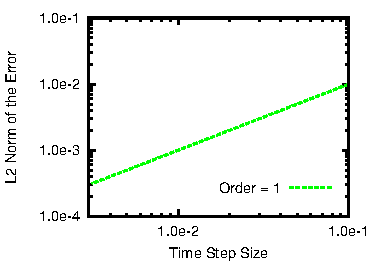
\includegraphics[scale=1.5]{figures/ForwardEuler}\caption{Order of accuracy for the SinCos Problem (Section~\ref{rythmos:sec:SinCos-Problem})
using Forward Euler.\label{rythmos:fig:OrderofAccuracy-ForwardEuler}}
\end{figure}


\subsection{Explicit Runge-Kutta Methods\label{rythmos:sec:Explicit-Runge-Kutta-Methods}}

The general Runge-Kutta method for $s$-stages, can be written as
\[
X_{i}=x_{n-1}+\Delta t\,\sum_{j=1}^{s}a_{ij}\,\bar{f}(X_{j},t_{n-1}+c_{j}\Delta t)
\]
\[
x_{n}=x_{n-1}+\Delta t\,\sum_{i=1}^{s}b_{i}\,\bar{f}(X_{i},t_{n-1}+c_{i}\Delta t)
\]
where $X_{i}$ are intermediate approximations to the solution at
times, $t_{n-1}+c_{i}\Delta t$, (\emph{stage solutions}) which may
be correct to a lower order of accuracy than the solution, $x_{n}$.
We should note that these lower-order approximations are combined
through $b_{i}$ so that error terms cancel out and produce a more
accurate solution \cite[p. 80]{AscherPetzold}. One can also write
this in terms of $\dot{X}_{i}$ (or $\bar{f}(x,t)$)
\[
\dot{X}_{i}=\bar{f}\left(x_{n-1}+\Delta t\,\sum_{j=1}^{s}a_{ij}\,\dot{X}_{j},t_{n-1}+c_{i}\Delta t\right)
\]
\[
x_{n}=x_{n-1}+\Delta t\,\sum_{i=1}^{s}b_{i}\,\dot{X}_{i}
\]

A convenient method to convey Runge-Kutta methods is to use the Butcher
Tableau, which displays the coefficients in a ``table'' form.
\begin{table}[H]
\caption{Schematic for a Butcher Tableau.\label{rythmos:tab:SchematicButcherTableau}}
\[
\begin{array}{c|cccc}
c_{1} & a_{11} & a_{12} & \ldots & a_{1s}\\
c_{2} & a_{21} & a_{22} & \ldots & a_{2s}\\
\vdots & \vdots & \vdots & \ddots & \vdots\\
c_{s} & a_{s1} & a_{s2} & \ldots & a_{ss}\\
\hline  & b_{1} & b_{2} & \ldots & b_{s}
\end{array}
\]
\end{table}
Notes:
\begin{enumerate}
\item $c_{i}$ is the fractional time step that the approximate solution
$X_{i}$ is known. It is possible for $c_{i}$ to be outside the time
step range {[}0,1{]}, however it is odd for a One-Step methods like
Runge-Kutta to have stage solutions outside the current time step. 
\item $c_{i}=\sum_{j=1}^{s}a_{ij}$ for $i=1,\ldots,s$
\item For explicit methods, \emph{e.g.}, Forward Euler and Explicit RK4,
$c_{1}=0$ and $a_{1j}=0$ for all $j$ indicates that one needs the
solution, $x_{n-1}$, and its time derivative, $\dot{x}_{n-1}$, (or
basically an evaluation of $\bar{f}(x_{n-1},t_{n-1})$) to start the
time step.
\item If $a_{ij}=0$ for $j\ge i$, the Runge-Kutta (RK) method is explicit
(also known as ERK), since each $X_{i}$ is given in terms of known
quantities.
\item If $a_{ij}\ne0$ for any $j\ge i$, the Runge-Kutta (RK) method is
implicit (also known as IRK), since an implicit solve is required
for at least some of the stages.
\item If $a_{ij}=0$ for $j>i$, the method is known as a Diagonally Implicit
Runge-Kutta (DIRK) method. DIRK methods require an implicit solution
for each stage, but are not coupled to other stages.
\item If $a_{ij}=0$ for $j>i$ and $a_{ii}=C$, the method is known as
a Singly Diagonally Implicit Runge-Kutta (SDIRK) method. Like with
DIRK methods, an implicit solve is needed at each stage, but since
$a_{ii}$ is the same, some of the preparatory calculations can be
reused for each stage.
\item $b_{i}$ are the weighting of the intermediate solutions, $X_{i}$,
to obtain the final solution, and they are a partition of unity, $\sum_{i=1}^{s}b_{i}=1$.
\item If $a_{sj}=b_{j}$ for all $j$ or $a_{i1}=b_{1}$ for all $i$, and
$a_{ij}$ is a nonsingular matrix, then A-stable RK methods are L-stable
\cite[p. 45]{HairerWanner}\cite[p. 103]{AscherPetzold}, \emph{e.g.},
Backward Euler and two SDIRK methods. Each of the above conditions
are not a necessary condition for L-stability, but they are a sufficient
condition.
\end{enumerate}

\subsection{Explicit RK Forward Euler}

Forward Euler can also be written for Runge-Kutta methods, Fig.~\ref{rythmos:fig:ERK-ForwardEuler},
and obtains convergence results similar to Forward Euler, Section~\ref{rythmos:sec:Forward-Euler}.
\begin{figure}[H]
\centering{}%
\begin{tabular}{cc}
a)$\begin{array}{c|c}
0 & 0\\
\hline  & 1
\end{array}$ & b)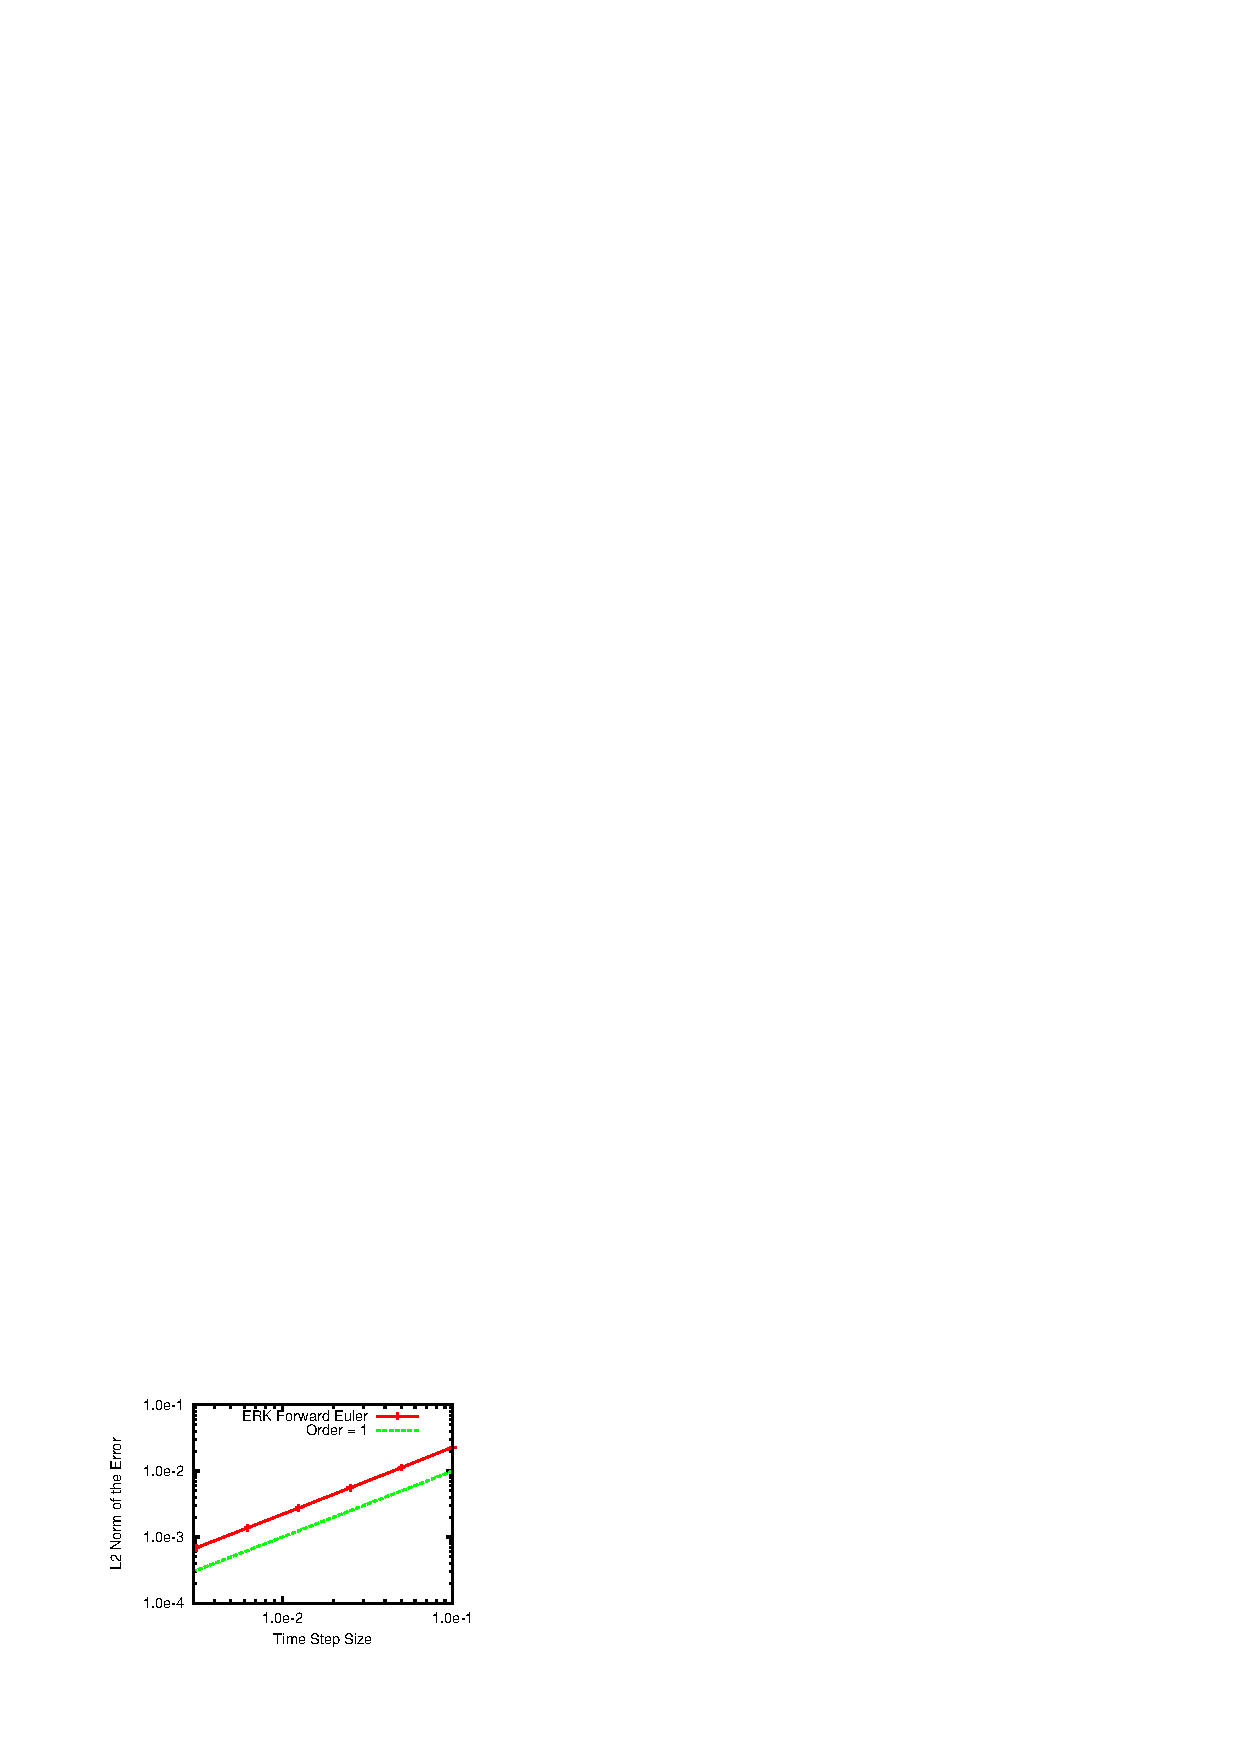
\includegraphics[scale=1.5]{figures/ERK_ForwardEuler}\tabularnewline
\end{tabular}\caption{a) Butcher Tableau and b) Order of accuracy for the SinCos Problem
(Section~\ref{rythmos:sec:SinCos-Problem}) for Explicit RK Forward
Euler.\label{rythmos:fig:ERK-ForwardEuler}}
\end{figure}


\subsection{Explicit RK 2 Stage 2 Order by Runge (Explicit Midpoint)}

\begin{figure}[H]
\centering{}%
\begin{tabular}{cc}
a) $\begin{array}{c|cc}
0 & 0\\
1/2 & 1/2 & 0\\
\hline  & 0 & 1
\end{array}$ & b)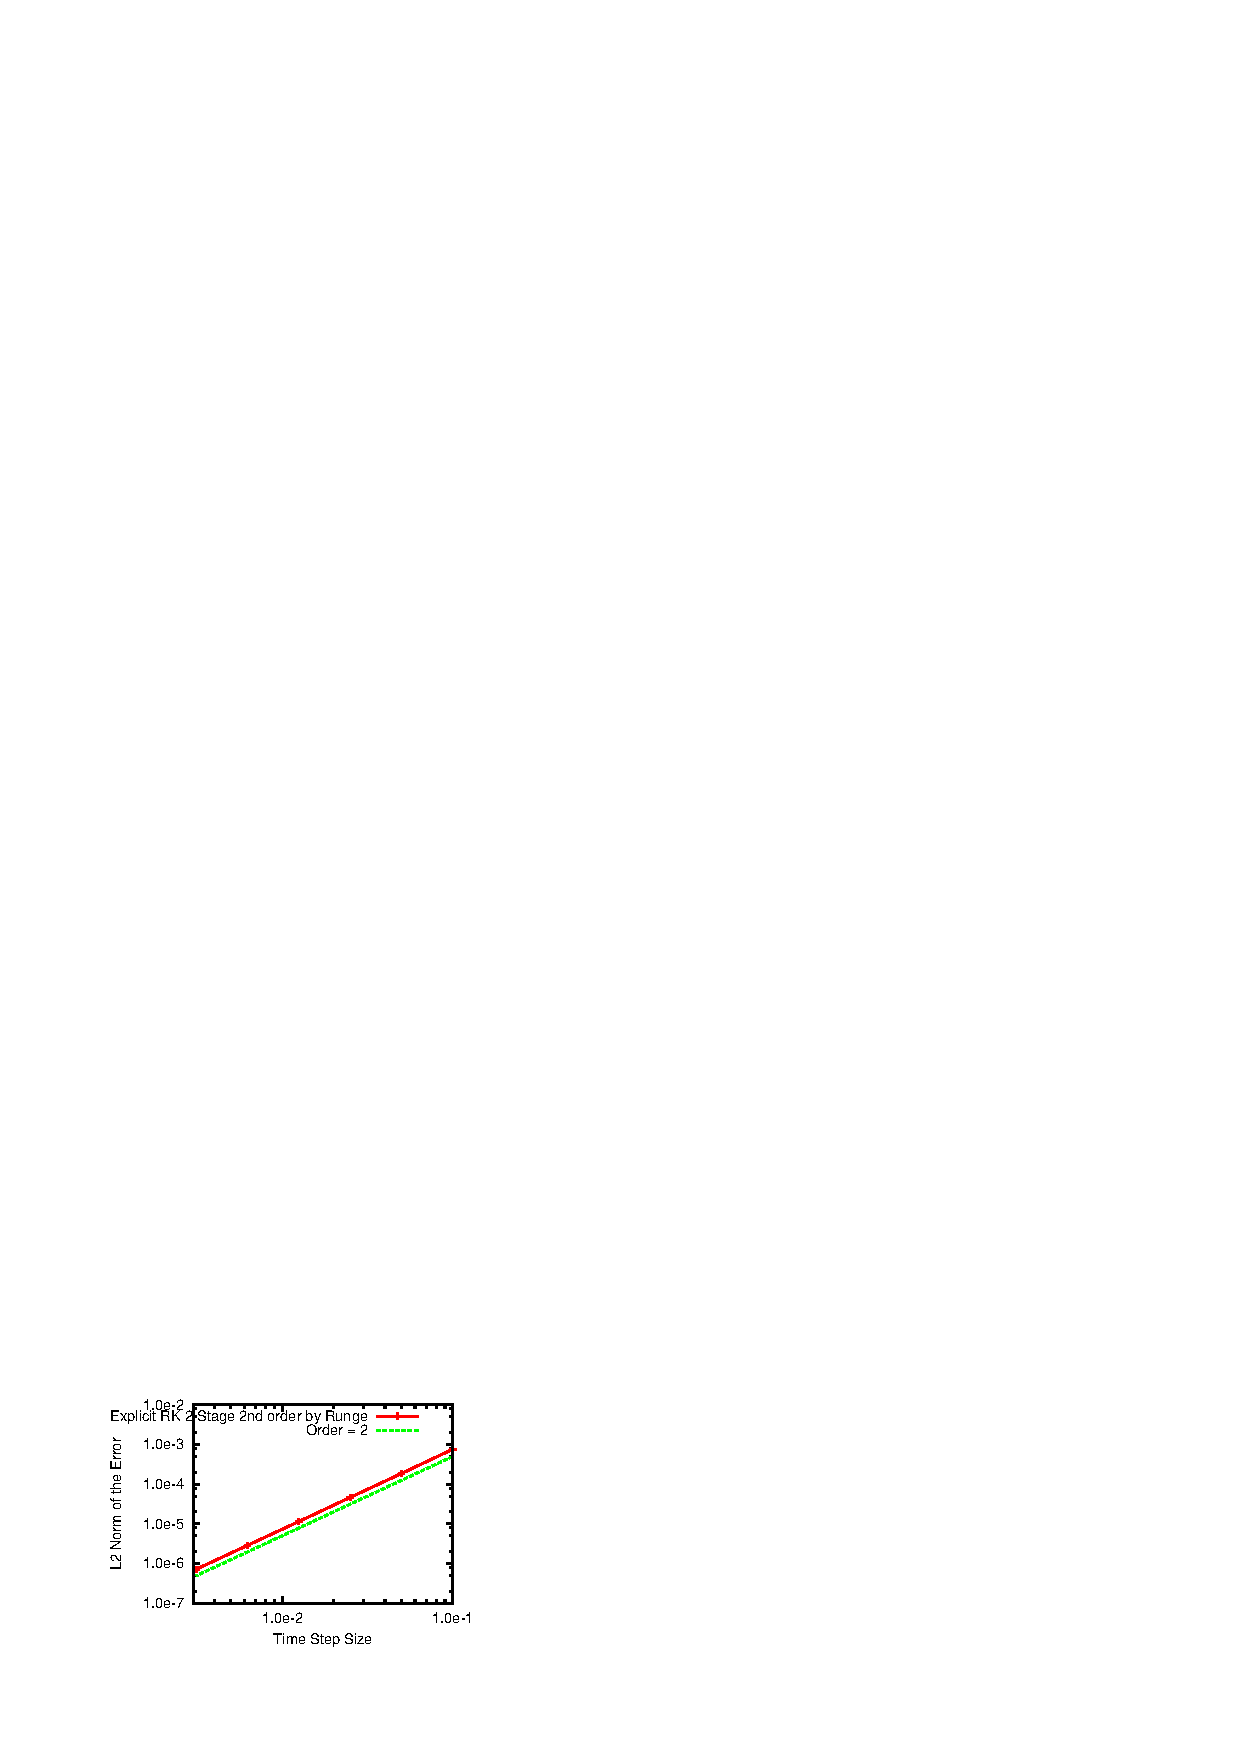
\includegraphics[scale=1.5]{figures/ERK_2Stage2OrderRunge}\tabularnewline
\end{tabular}\caption{a) Butcher Tableau and b) Order of accuracy for the SinCos Problem
(Section~\ref{rythmos:sec:SinCos-Problem}) for Explicit RK 2 Stage
2nd Order by Runge.\label{rythmos:tab:ButcherTableau-ERK_2Stage2OrderRunge}.}
\end{figure}


\subsection{Explicit RK Trapezoidal}

\begin{figure}[H]
\centering{}%
\begin{tabular}{cc}
a) $\begin{array}{c|cc}
0 & 0\\
1 & 1 & 0\\
\hline  & 1/2 & 1/2
\end{array}$ & b)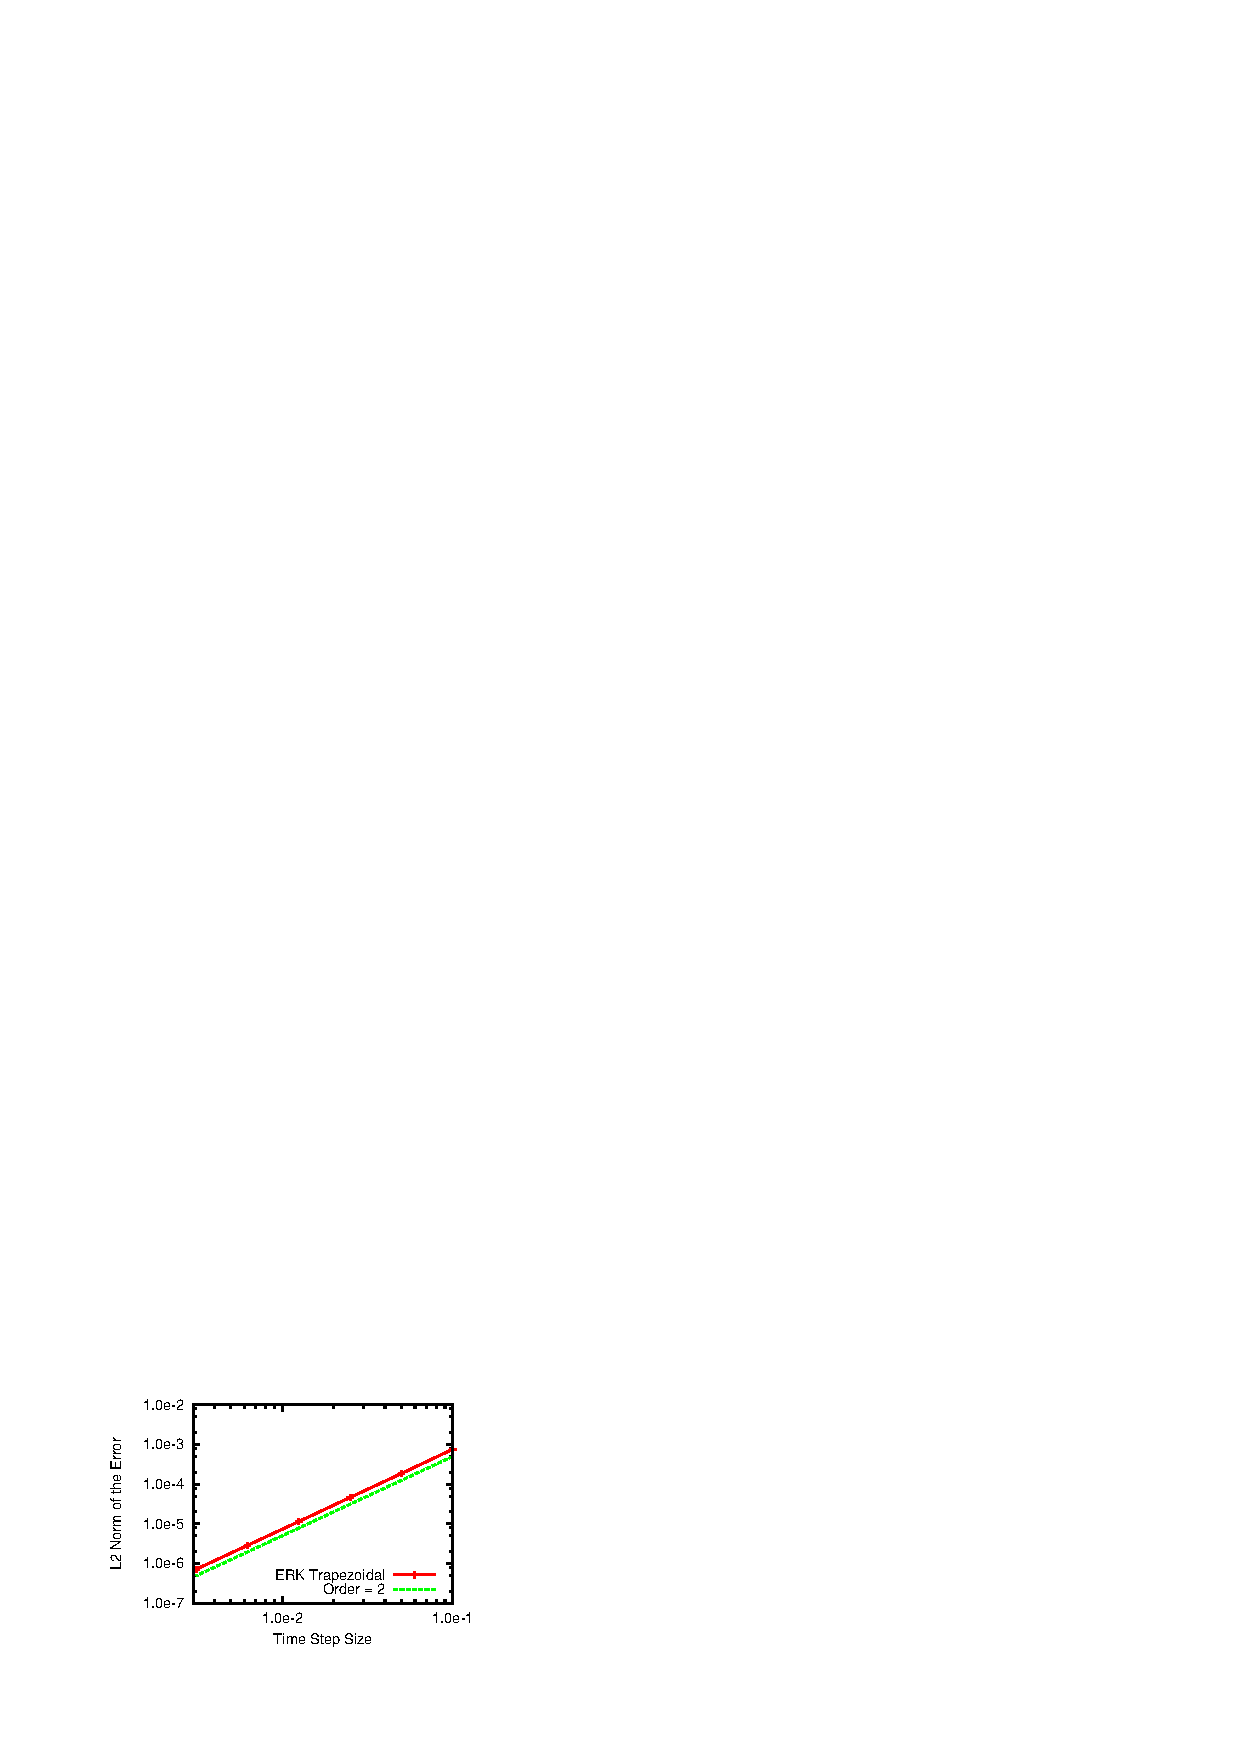
\includegraphics[scale=1.5]{figures/ERK_Trapezoidal}\tabularnewline
\end{tabular}\caption{a) Butcher Tableau and b) Order of accuracy for the SinCos Problem
(Section~\ref{rythmos:sec:SinCos-Problem}) for Explicit RK Trapezoidal.\label{rythmos:tab:ButcherTableau-ERK_Trapezoidal}}
\end{figure}


\subsection{Explicit RK 3 Stage 3 Order}

\begin{figure}[H]
\centering{}%
\begin{tabular}{cc}
a)$\begin{array}{c|ccc}
0 & 0\\
1/2 & 1/2 & 0\\
1 & -1 & 2 & 0\\
\hline  & 1/6 & 4/6 & 1/6
\end{array}$ & b)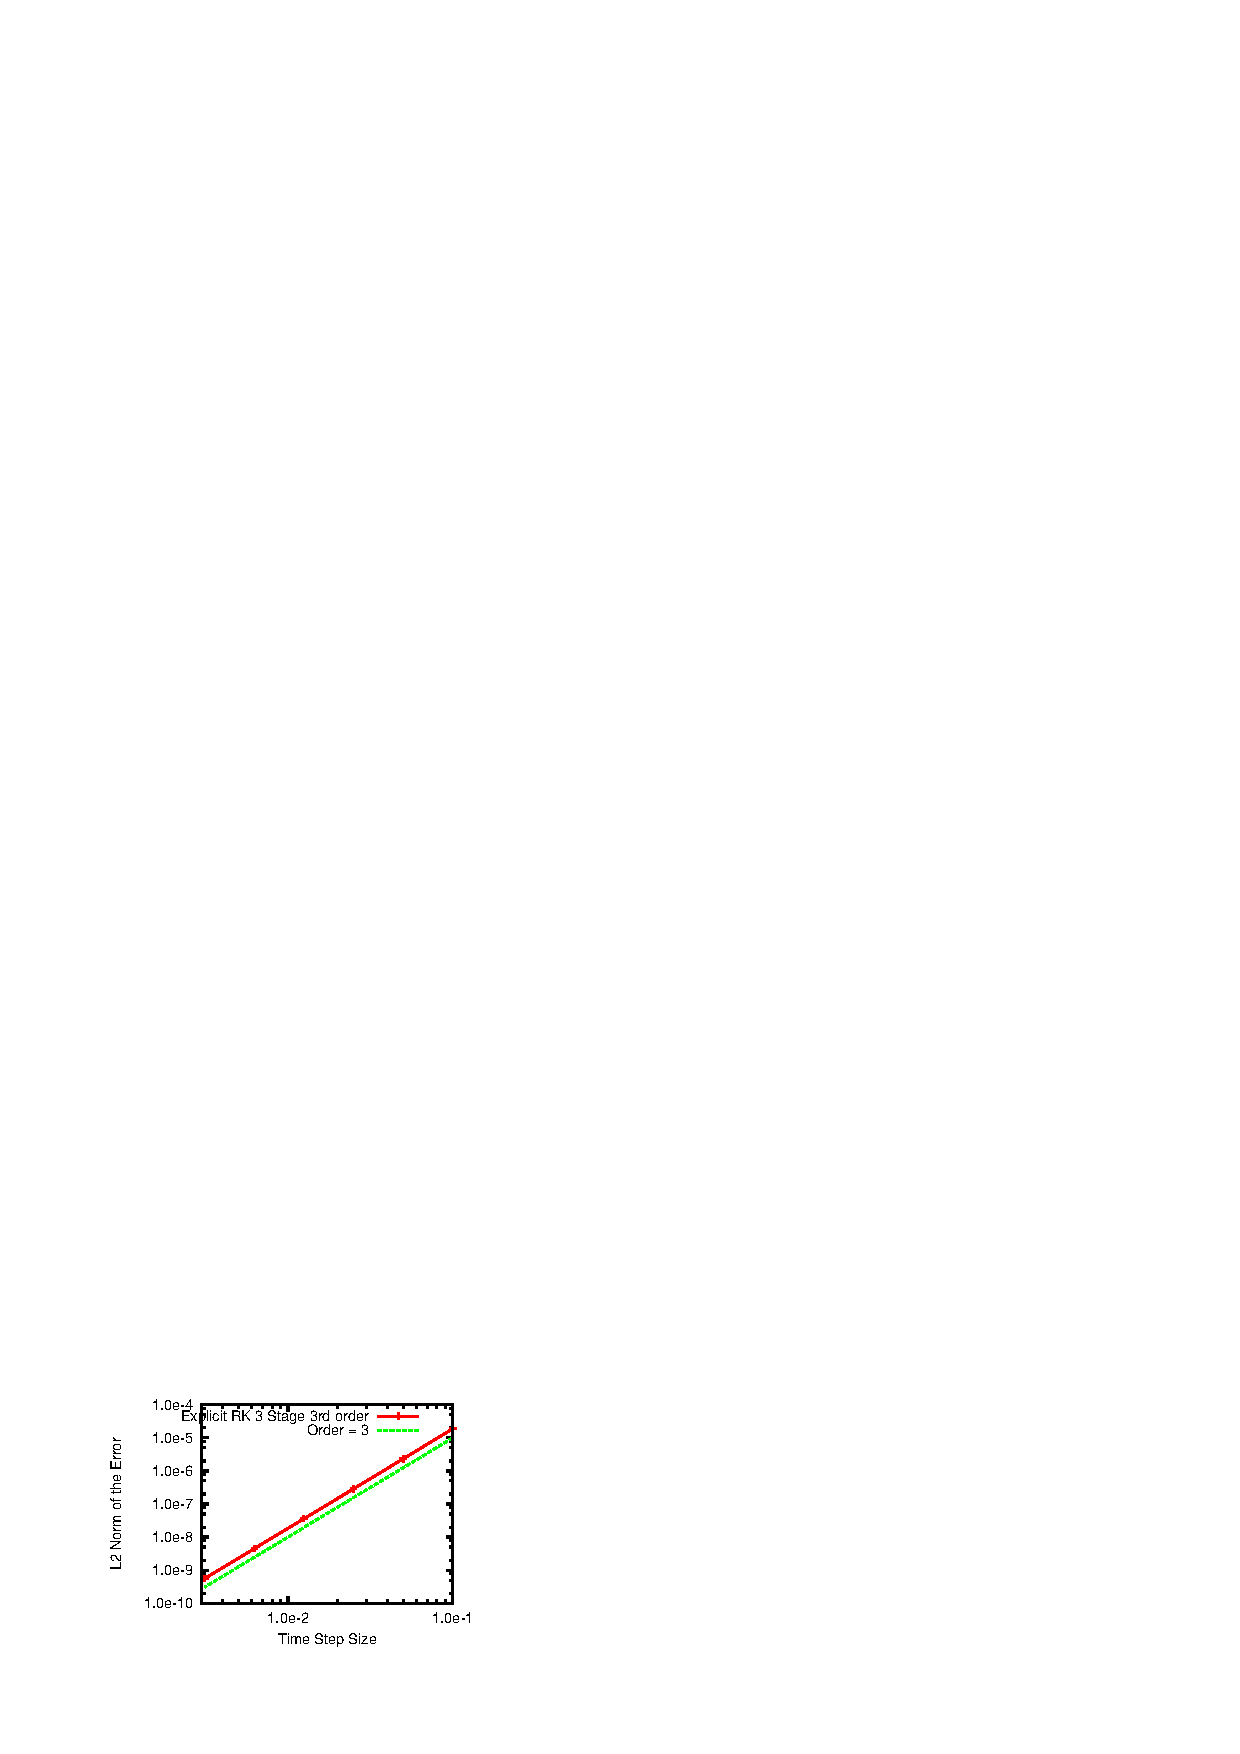
\includegraphics[scale=1.5]{figures/ERK_3Stage3Order}\tabularnewline
\end{tabular}\caption{a) Butcher Tableau and b) Order of accuracy for the SinCos Problem
(Section~\ref{rythmos:sec:SinCos-Problem}) for Explicit RK 3 Stage
3rd Order.\label{rythmos:tab:ButcherTableau-ERK_3Stage3Order}}
\end{figure}


\subsection{Explicit RK 3 Stage 3 Order by Heun}

\begin{figure}[H]
\centering{}%
\begin{tabular}{cc}
a) $\begin{array}{c|ccc}
0 & 0\\
1/3 & 1/3 & 0\\
2/3 & 0 & 2/3 & 0\\
\hline  & 1/4 & 0 & 3/4
\end{array}$ & b)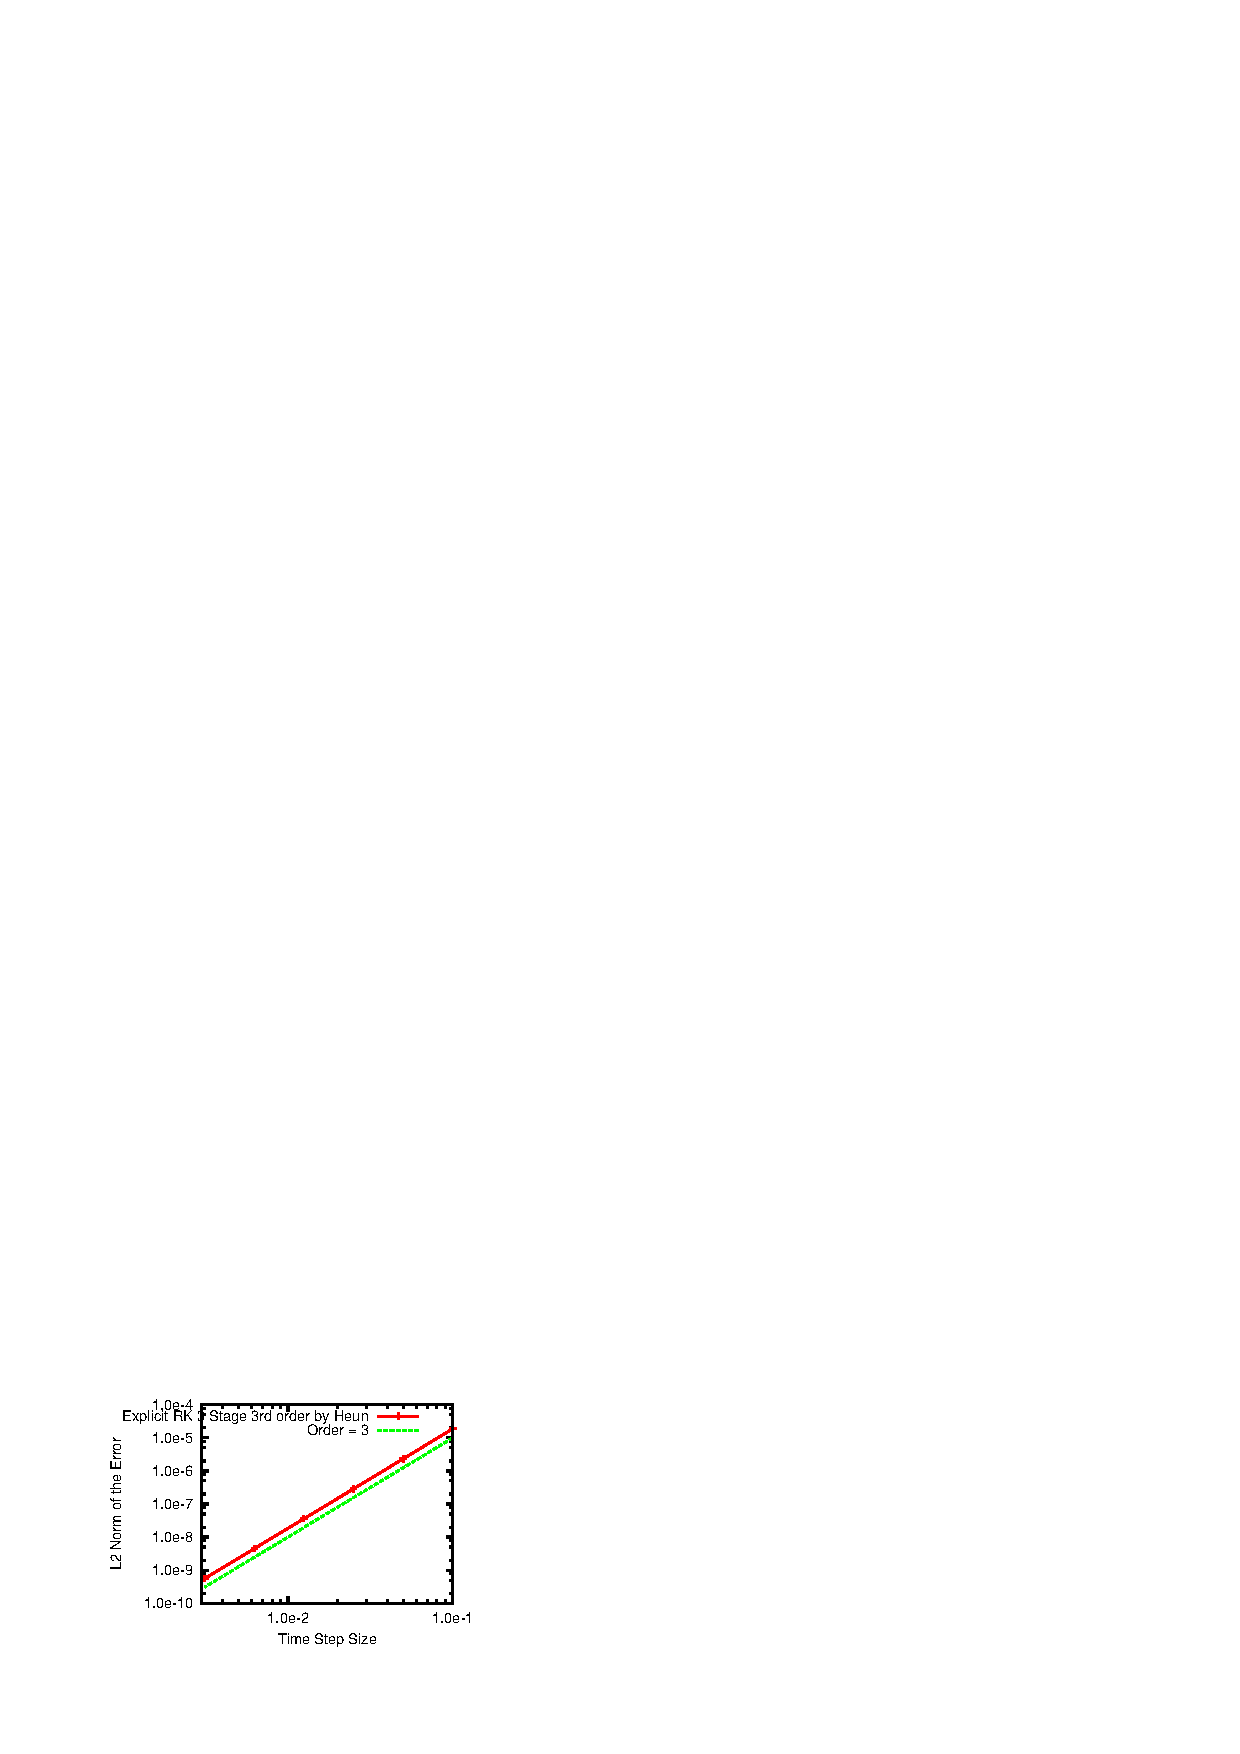
\includegraphics[scale=1.5]{figures/ERK_3Stage3OrderHeun}\tabularnewline
\end{tabular}\caption{a) Butcher Tableau and b) Order of accuracy for the SinCos Problem
(Section~\ref{rythmos:sec:SinCos-Problem}) for Explicit RK 3 Stage
3rd Order by Heun.\label{rythmos:tab:ButcherTableau-ERK_3Stage3OrderHeun}}
\end{figure}


\subsection{Explicit RK 3 Stage 3 Order TVD}

\begin{figure}[H]
\centering{}%
\begin{tabular}{cc}
a)$\begin{array}{c|ccc}
0 & 0\\
1 & 1 & 0\\
1/2 & 1/4 & 1/4 & 0\\
\hline  & 1/6 & 1/6 & 4/6
\end{array}$ & b)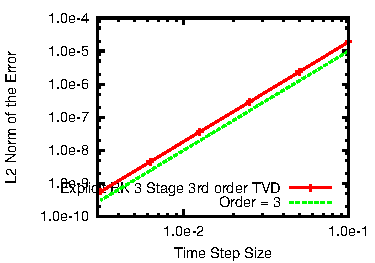
\includegraphics[scale=1.5]{figures/ERK_3Stage3OrderTVD}\tabularnewline
\end{tabular}\caption{a) Butcher Tableau and b) Order of accuracy for the SinCos Problem
(Section~\ref{rythmos:sec:SinCos-Problem}) for Explicit RK 3 Stage
3rd Order TVD.\label{rythmos:tab:ButcherTableau-ERK_3Stage3OrderTVD}}
\end{figure}


\subsection{Explicit RK 4 Stage 3 Order by Runge}

\begin{figure}[H]
\centering{}%
\begin{tabular}{cc}
a)$\begin{array}{c|cccc}
0 & 0\\
1/2 & 1/2 & 0\\
1 & 0 & 1 & 0\\
1 &  & 0 & 1 & 0\\
\hline  & 1/6 & 2/3 & 0 & 1/6
\end{array}$ & b)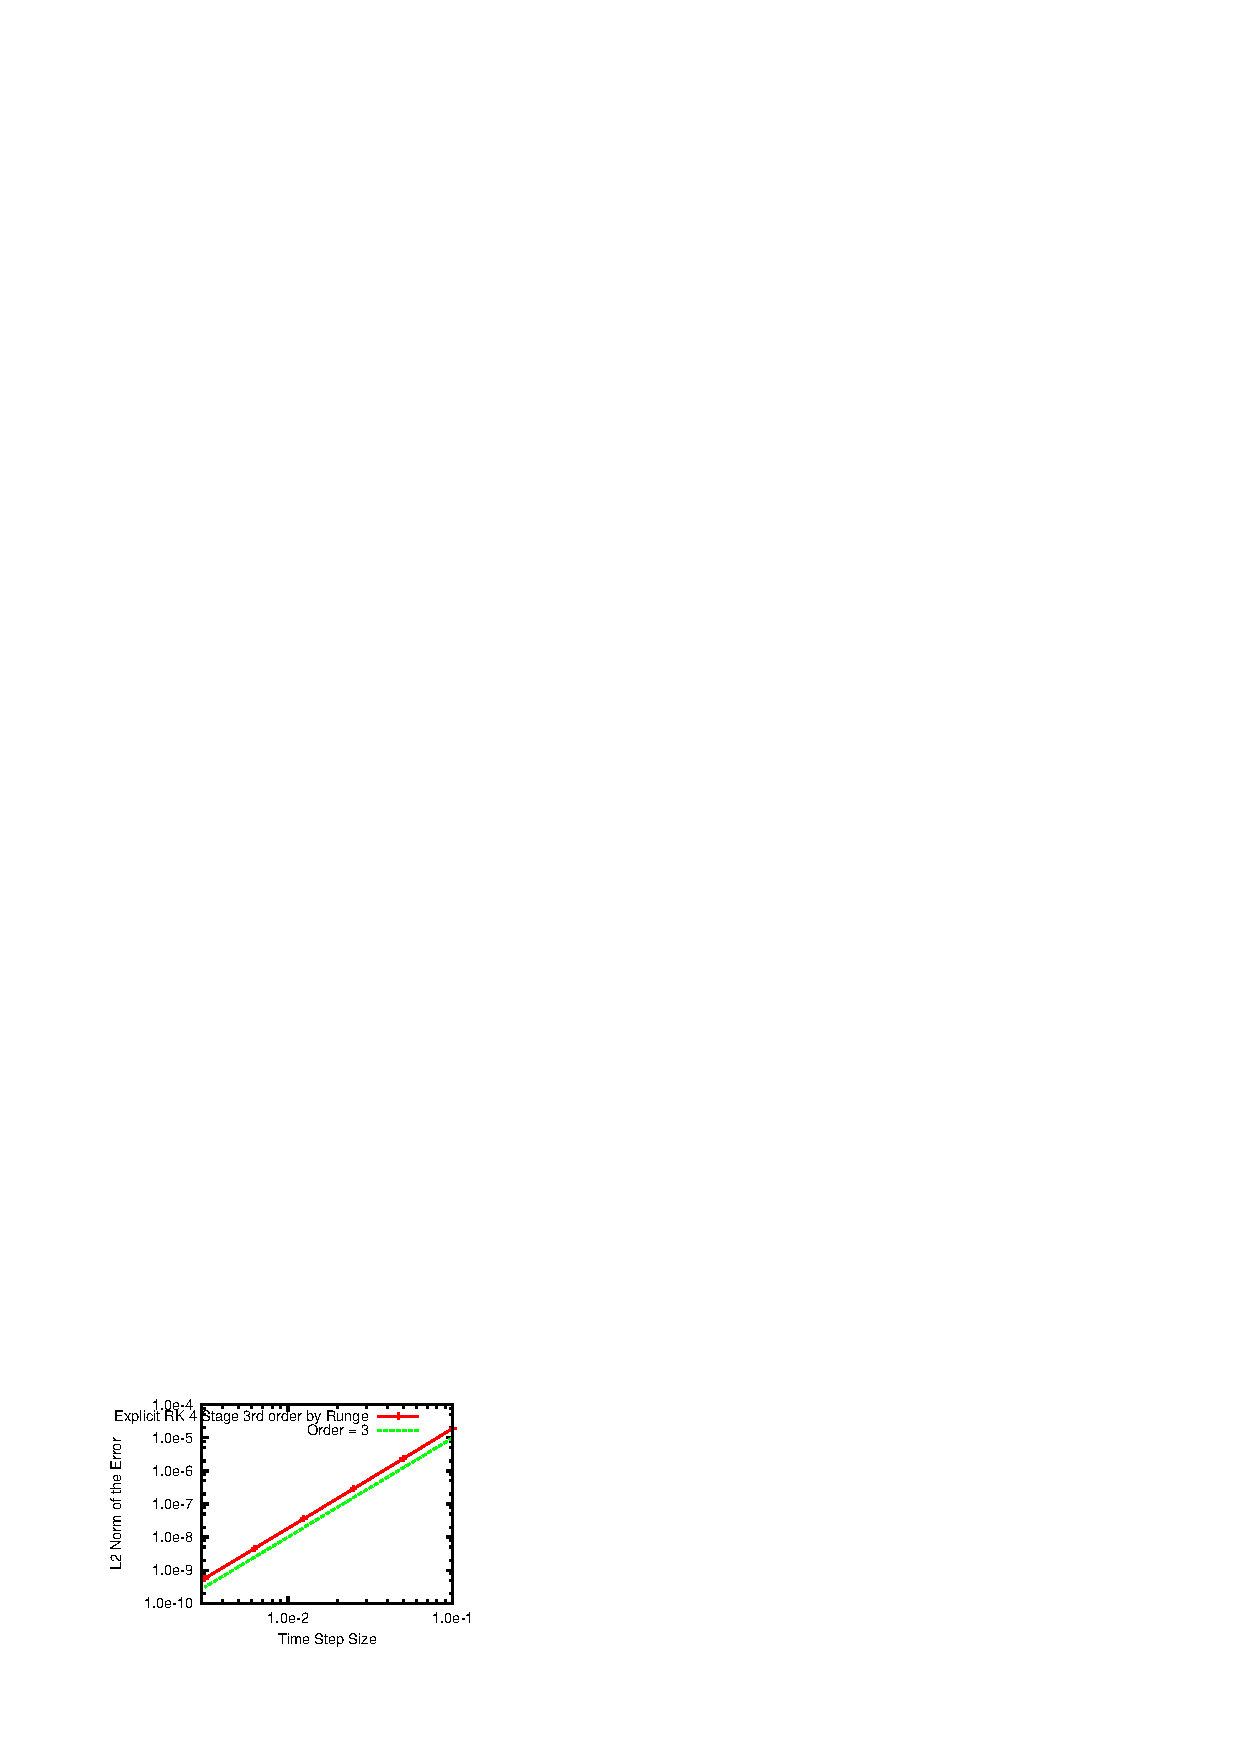
\includegraphics[scale=1.5]{figures/ERK_4Stage3OrderRunge}\tabularnewline
\end{tabular}\caption{a) Butcher Tableau and b) Order of accuracy for the SinCos Problem
(Section~\ref{rythmos:sec:SinCos-Problem}) for Explicit RK 4 Stage
3rd Order by Runge.\label{rythmos:tab:ButcherTableau-ERK_4Stage3OrderRunge}}
\end{figure}


\subsection{Explicit RK4}

\begin{figure}[H]
\centering{}%
\begin{tabular}{cc}
a)$\begin{array}{c|cccc}
0 & 0\\
1/2 & 1/2 & 0\\
1/2 & 0 & 1/2 & 0\\
1 & 0 & 0 & 1 & 0\\
\hline  & 1/6 & 1/3 & 1/3 & 1/6
\end{array}$ & b)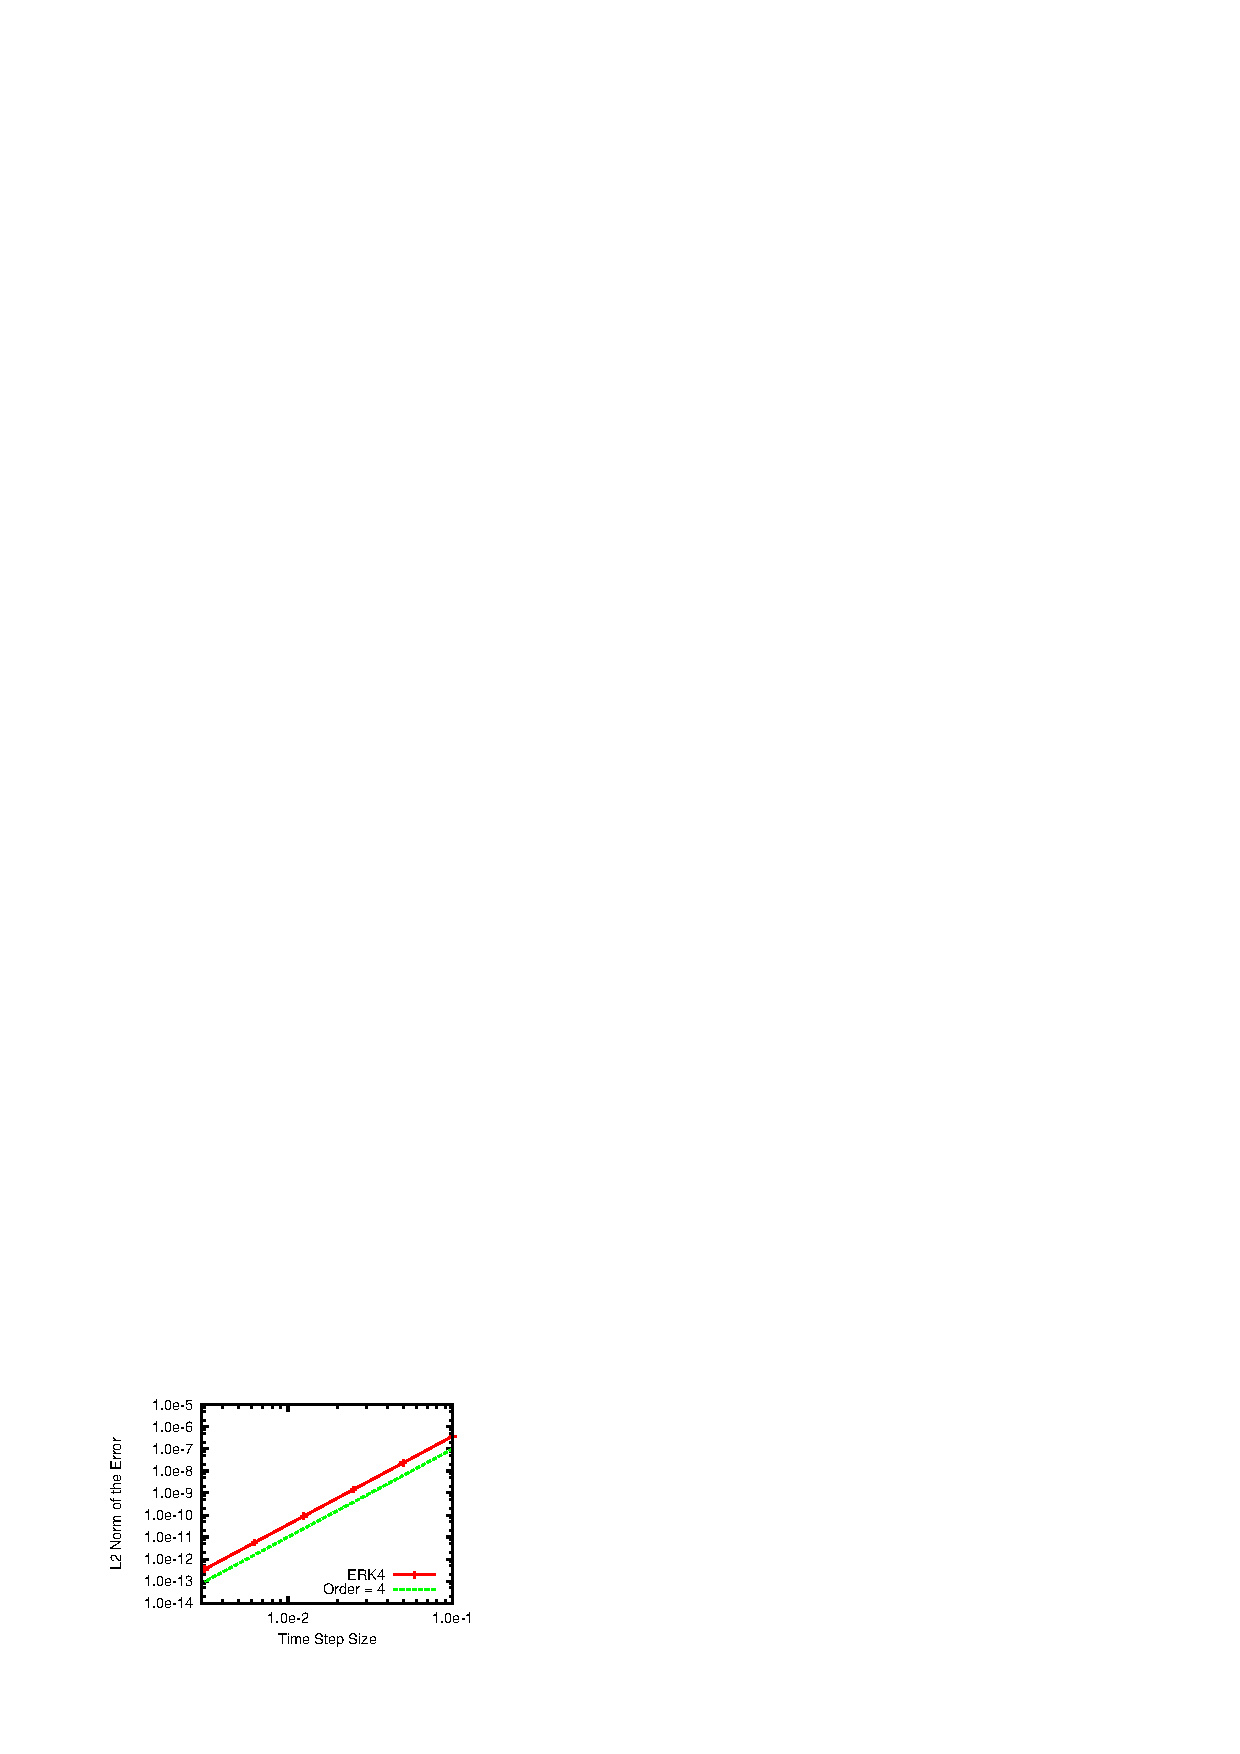
\includegraphics[scale=1.5]{figures/ERK_4Stage}\tabularnewline
\end{tabular}\caption{a) Butcher Tableau and b) Order of accuracy for the SinCos Problem
(Section~\ref{rythmos:sec:SinCos-Problem}) for Explicit RK 4.\label{rythmos:tab:ButcherTableau-ERK_4Stage}.}
\end{figure}


\subsection{Explicit RK 3/8 Rule}

\begin{figure}[H]
\centering{}%
\begin{tabular}{cc}
a)$\begin{array}{c|cccc}
0 & 0\\
1/3 & 1/3 & 0\\
2/3 & -1/3 & 1 & 0\\
1 & 1 & -1 & 1 & 0\\
\hline  & 1/8 & 3/8 & 3/8 & 1/8
\end{array}$ & b)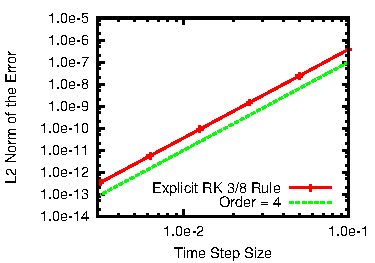
\includegraphics[scale=1.5]{figures/ERK_3_8_Rule}\tabularnewline
\end{tabular}\caption{a) Butcher Tableau and b) Order of accuracy for the SinCos Problem
(Section~\ref{rythmos:sec:SinCos-Problem}) for Explicit RK 3/8 Rule.\label{rythmos:tab:ButcherTableau-ERK_3_8_Rule}}
\end{figure}

